
\includegraphics[height=1.25cm]{images/pictograms/FEM}
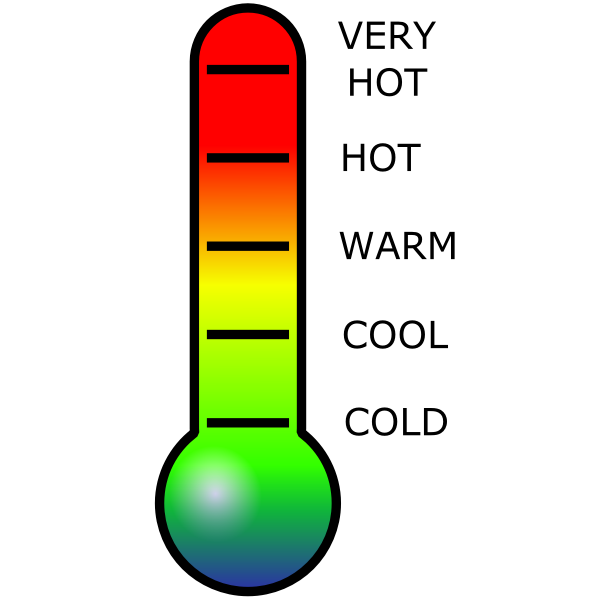
\includegraphics[height=1.25cm]{images/pictograms/temperature}

\includegraphics[height=1.25cm]{images/pictograms/nonlinear}

\includegraphics[height=1.25cm]{images/pictograms/publication}

%%%%%%%%%%%%%%%%%%%%%%%%%%%%%%%%%%%%%%%%%%%%%%%%%%%%%%%%%%%%%%%%%%%%%%%%%%%%%%%%%%%%%%%%%%%%%%%%%%%

\begin{flushright} {\tiny {\color{gray} python\_codes/fieldstone\_50/text.tex}} \end{flushright}

\lstinputlisting[language=bash,basicstyle=\small]{python_codes/fieldstone_50/keywords.key}

\begin{center}
Code at \url{https://github.com/cedrict/fieldstone/tree/master/python_codes/fieldstone_50}
\end{center}

\par\noindent\rule{\textwidth}{0.4pt}

{\sl The setup for this stone comes from J. Naliboff}. 
\index{contributors}{J. Naliboff} \index{contributors}{J. Naliboff}

\par\noindent\rule{\textwidth}{0.4pt}
%%%%%%%%%%%%%%%%%%%%%%%%%%%%%%%%%%%%%%%%%%%%%%%%%%%%%%%%%%%%%%%%%%%%%%%%%%%%%%%%%%%%%%%%%%%%


The code is based on quadrilateral $Q_2\times Q_1$ elements.
The domain is $400~\si{\km}\times 100~\si{km}$ and the 
mesh is composed of $160\times 40$ elements. Gravity is Earth-like.
There are 4 materials in the domain:
\begin{itemize}
\item upper crust (20~\si{\km} thick layer)
\item lower crust (10~\si{\km} thick layer)
\item mantle lithosphere (70~\si{\km} thick layer)
\item weak seed for $60<y<68$km and $198<x<202$km
\end{itemize}
Each element is assigned a material number ('imat'). 
The rheology is visco-plastic, with a dislocation creep rheology for the viscous branch and 
a Drucker-Prager yield criterion. Nonlinear (Picard) iterations are carried out until 
a relative tolerance $tol=10^{-4}$ is reached. TODO!!!
The viscosity and density are computed at each quadrature point.
For visualisation purposes these are averaged per element.
 
Kinematical boundary conditions are precribed on the sides and bottom boundaries:
$u=-0.25~\si{\cm\per\year}$ on the left, 
$u=+0.25~\si{\cm\per\year}$ on the right, 
and $v=+0.125~\si{\cm\per\year}$ on the bottom. 

The temperature field is piecewise linear in the $y$-direction: from 
0~\si{\celsius} to 500~\si{\celsius} at 30~\si{\km} depth, and then to 1500~\si{\celsius} at the bottom. 
Pressure $p$ is interpolated onto the velocity node ($q$ field).
There is no time stepping and the heat transport equation is not solved.

Results are exported to vtu format (solution.vtu) but also by means of 
matplotlib (solution.pdf). Note that I'd be happy if anybody knows how to 
fix the size of the colorbars.	

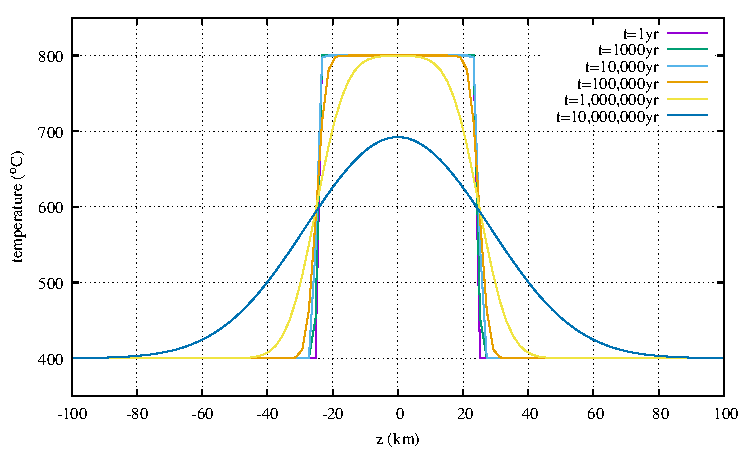
\includegraphics[width=16cm]{python_codes/fieldstone_50/images/solution.pdf}

For simplicity I compute the following convergence indicators:
\[
\xi_u=\frac{|| \vec{\cal U}^k-\vec{\cal U}^{k-1}||_2 }{||\vec{\cal U}^k+\vec{\cal U}^{k-1}||_2 }
\]
\[
\xi_v=\frac{|| \vec{\cal V}^k-\vec{\cal V}^{k-1}||_2 }{||\vec{\cal V}^k+\vec{\cal V}^{k-1}||_2 }
\]
\[
\xi_p=\frac{|| \vec{\cal P}^k-\vec{\cal P}^{k-1}||_2 }{||\vec{\cal P}^k+\vec{\cal P}^{k-1}||_2 }
\]
where $k$ denotes the nonlinear loop increment and $\vec{\cal U},\vec{\cal V},\vec{\cal P}$ 
denote the solution vectors. 
When/if the fields converge then the denominator converges to a 
single non-zero value and the numerator goes to zero.



\newpage
%%%%%%%%%%%%%%%%%%%%%%%%%%%%%%%%%%%%%%%%%%%%%%%%%%%%%%%%%%%%%%%%%%%%%%%%%%%%%%%%%%%%%%
\section*{Relaxing the viscosity}

As an experiment, I have implemented a simple relaxation scheme on the nonlinear viscosity.
At each iteration the newly computed viscosity at a quadrature point is weighed by a factor
$\gamma$ and added to the previously obtained viscosity weighed by a factor $(1-\gamma)$.

\begin{lstlisting}
etaq[counterq]=etaq[counterq]*gamma_eta+(1-gamma_eta)*etaq_mem[counterq]
\end{lstlisting}

If $\gamma=1$ then no relaxation takes place.
Convergence results are shown in the following figure:

\begin{center}
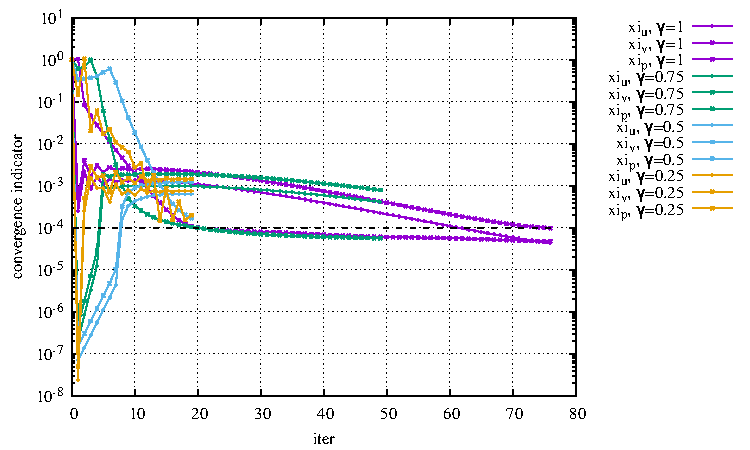
\includegraphics[width=8cm]{python_codes/fieldstone_50/results/conv_eta.pdf}
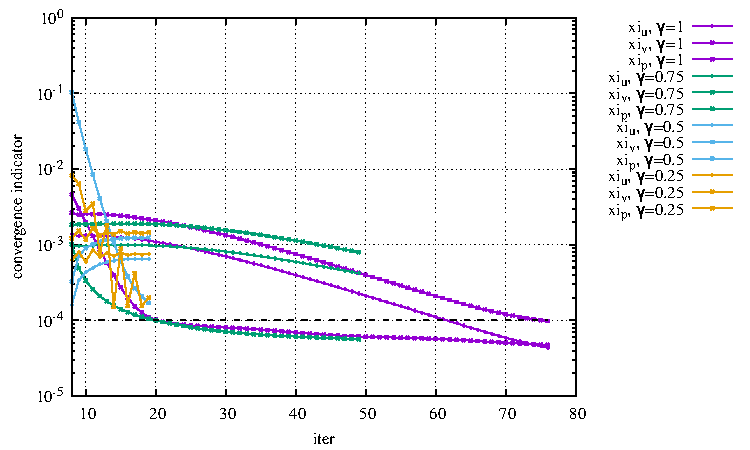
\includegraphics[width=8cm]{python_codes/fieldstone_50/results/conv_eta_zoom.pdf}\\
{\captionfont $\eta_{ref}=10^{23}$. Note that I have not run all simulations 
to convergence.}
\end{center}

We see that 1) all curves seem to plateau first and then seem to converge very slowly; 
b) this relaxation scheme does not improve things much at all...

Let us explore the parameters which could alter these convergence results
and let us start with the reference viscosity. Changing it to 1e21 does not 
alter the results.  

%%%%%%%%%%%%%%%%%%%%%%%%%%%%%%%%%%%%%%%%%%%%%%%%%%%%%%%%%%%%%%%%%%%%%%%%%%%%%%%%%%%%%%
\section*{Relaxing the velocity and pressure}

The same approach is now taken for the velocity and pressure (while the viscosity is left alone).

\begin{lstlisting}
u=u*gamma_uvp+u_old*(1-gamma_uvp)
v=v*gamma_uvp+v_old*(1-gamma_uvp)
p=p*gamma_uvp+p_old*(1-gamma_uvp)
\end{lstlisting}


\begin{center}
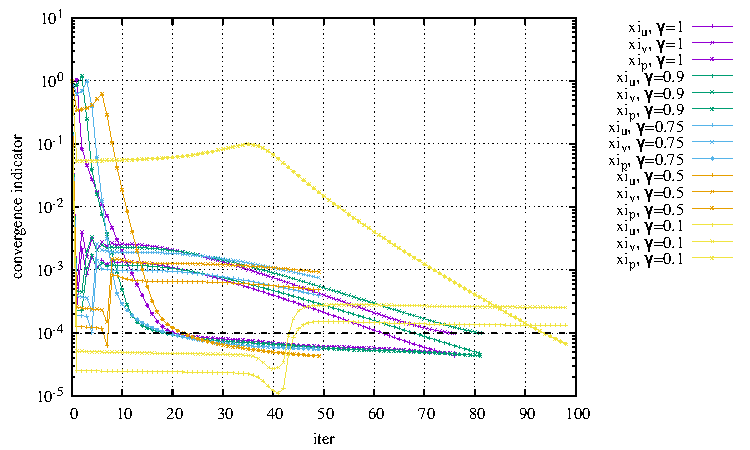
\includegraphics[width=8cm]{python_codes/fieldstone_50/results/conv_uvp.pdf}
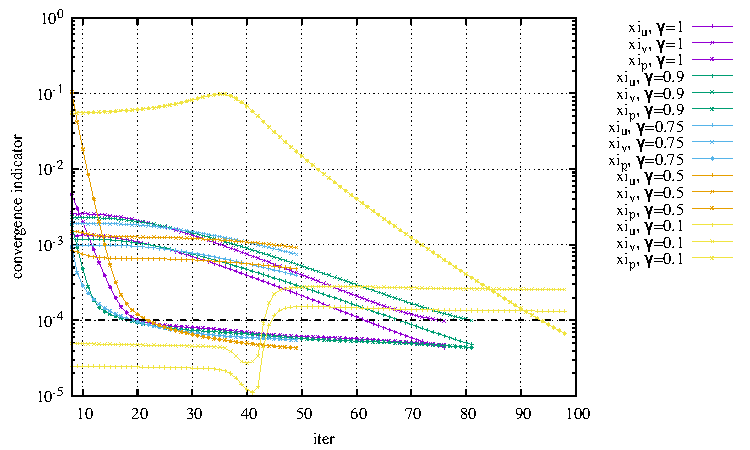
\includegraphics[width=8cm]{python_codes/fieldstone_50/results/conv_uvp_zoom.pdf}
\end{center}

As before we can conclude that such simple relaxation scheme does not substantially 
improve (if at all) the convergence.

%%%%%%%%%%%%%%%%%%%%%%%%%%%%%%%%%%%%%%%%%%%%%%%%%%%%%%%%%%%%%%%%%%%%%%%%%%%%%%%%%%%%%%%%%%%%%%%%%%%
\par\noindent\rule{\textwidth}{0.4pt}

\vspace{.5cm}

\begin{center}
\fbox{\begin{minipage}{0.9\textwidth}
{\color{teal}To Do, open questions, future work?}
\begin{itemize}
\item compute nonlinear residuals instead of $\xi$ vallues 
\item extract velocity and/or pressure value at key points and monitor as a function of the nonlinear iterations loop increment
\end{itemize}
\end{minipage}}
\end{center}





